\section{Control Dinámico del brazo}
En esta última parte del proyecto, una vez se conoce el modelo del robot en las diferentes configuraciones, se pasará a buscar implementar un control dinámico sobre el mismo.Para poder implementar controladores sobre nuestro robot, será necesario obtener una función de transferencia matemática a modo de modelo que se asemeje al robot real.\\
Una vez se tenga un modelo lineal de cada articulación del robot, junto con el generador de trayectorias creado anteriormente, se buscará que el robot siga una trayectoria predefinida. Básicamente, se busca que el robot se desplace de un punto a otro minimizando el error y del modo y a la velocidad que el usuario desee.\\

	\subsection{Obtención del modelo lineal de las articulaciones del brazo}
Para obtener la función de transferencia de cada articulación del robot, se linealizará la ecuación dinamica que define cada motor en un punto de equilibrio en torno a velocidades nulas. Por lo tanto, las consideraciones que se tendrán en cuenta para linealizar la ecuación dinamica que define el comportamiento de cada articulacion del robot son:
\begin{itemize}
	\item Velocidades de equilibrio
	\begin{center}
		$ \dot{q_{eq}}=0 rad/s $\\
		$ \dot{q} =\dot{q_{eq}}+\Delta\dot{q}$
	\end{center}
	\item Aceleraciones de equilibrio
\begin{center}
	$ \ddot{q_{eq}}=0 rad/s $\\
	$  $
	$ \ddot{q} =\ddot{q_{eq}}+\Delta\ddot{q}$
\end{center}
\end{itemize}

Ademas de ello, se aplicarán una serie de simplificaciones a la ecuación dinámica. A continuación, se mostrarán las ecuaciones dinámicas de los motores:\\
\begin{center}
	$$
	\begin{pmatrix}
	 \tau_{1} \\
	 \tau_{2} \\
	 \tau_ {3}
	\end{pmatrix}=
	\begin{pmatrix}
	Kt_{1}R_{1}Im_{1}  \\
	Kt_{2}R_{2}Im_{2}  \\
	Kt_{3}R_{3}Im_{3}
	\end{pmatrix} =
	\begin{pmatrix}
	Ma_{11} & Ma_{12} & Ma_{13}  \\
	Ma_{21} & Ma_{22} & Ma_{23}  \\
	Ma_{31} & Ma_{32} & Ma_{33}
	\end{pmatrix}
	\ddot{q}+
	\begin{pmatrix}
	Va_{1} \\
	Va_{2} \\
	Va_{3} \\
	\end{pmatrix}
	\dot{q}+
	\begin{pmatrix}
	Ga_{1}  \\
	Ga_{2}  \\
	Ga_{3}\\
	\end{pmatrix}
	$$
\end{center}
donde se asume que dentro de los términos de inercia y de Coirolis se han tenido en cuenta las inercias y fricciones viscosas de los motores.\\

La primera simplificación del modelo que se hará para poder linealizar el modelo en torno a un punto de operación, será suponer la matriz de inercias diagonal y, además de ello, se cogerá el valor medio de todos los senos y cosenos de tal modo que únicamente se tomen los valores de inercias medios. De manera praćtica, se harán cero todas las variables articulares del modelo. De éste modo, se desacoplará el sistema.\\
En cuando a la matriz de términos de Coirolis, únicamente aportarán a la linealización la fricción viscosa de los motores, es decir, se despreciarán todos los terminos exceptuando el que acompañe al valor de la velocidad articular.\\
Por último, la gravedad se despreciará para obtener un modelo, de tal modo que, se emplearán las siguientes ecuaciones para obtener los modelos de las articulaciones del robot:
\begin{equation}
	\begin{pmatrix}
	Kt_{1}R_{1}Im_{1}  \\
	Kt_{2}R_{2}Im_{2}  \\
	Kt_{3}R_{3}Im_{3}
	\end{pmatrix} =
	\begin{pmatrix}
	Ma_{11} & 0 	  & 0  \\
		0   & Ma_{22} & 0  \\
		0   & 0   	  & Ma_{33}
	\end{pmatrix}
	\ddot{q}+
	\begin{pmatrix}
	Va_{1} \\
	Va_{2} \\
	Va_{3} \\
	\end{pmatrix}
	\dot{q}
\end{equation}

A continuación, se obtendrá el modelo de la primera articulación y, el procedimiento será análogo para las restantes:
\begin{center}
	$Kt_{1}R_{1}Im_{1}(t)=Ma_{11}\ddot{q_{1}(t)} + Va_{1}\dot{q_{1}(t)}$
\end{center}
Se realizará una transformación al dominio de Laplace y, posteriormente, se expresará en forma de función de transferencia:
\begin{equation}
	Kt_{1}R_{1}Im_{1}(s)=s^{2}Ma_{11}q_{1}(s) + sVa_{1}q_{1}(s) \rightarrow \frac{q_{1}(s)}{Im_{1}(s)}=\frac{Kt_{1}R_{1}}{s(Ma_{11}s+Va_{1})}
\end{equation}

Por lo tanto, se definirá el modelo de cada articulación cómo:
\begin{equation}
	G_{1}(s)=\frac{Kt_{1}R_{1}}{s(Ma_{11}s+Va_{1})} \hspace{1cm} G_{2}(s)=\frac{Kt_{2}R_{2}}{s(Ma_{2}s+Va_{2})} \hspace{1cm} G_{3}(s)=\frac{Kt_{3}R_{3}}{s(Ma_{33}s+Va_{3})}
\end{equation}

	\subsection{Diseño de controladores}
	En éste apartado, se analizará cómo se hayarán los controladores que, posteriormente se implementarán sobre el robot para hacer que se desplace a lo largo de una trayectoria que se generará mediante el control cinemático.\\
	Cabe destacar que, en los controladores que se implementen junto con el compensador de gravedad, el de dinámica o el par calculado, la realimentación podrá ser por referencia, en lugar de emplear las medidas reales, de tal modo que se realimente con una señal sin ruido ni errores.\\
	\subsubsection{Controlador PD/PID}
	Para diseñar éstos controladores lineales, se empleará el modelo anteriormente mostrado y se implementarán directamente. El esquema de control será el esquema clásico de control, ya que éste tipo de controladores serán lo primeros en implementar y, por extensión, los más sencillos. \\
	La función de transferencia de los controladores a implementar será:\\
	\begin{equation}
		C(s)=K_{P}(T_{D}s+1) \hspace{2cm} C(s)=K_{P}\frac{T_{D}T_{I}s^{2}+T_{I}s+1}{T_{I}s}
	\end{equation}

	\subsubsection{Controlador PD/PID con compensación de gravedad}
	Para implementar éste controlador, se parte de la base de que, aunque la gravedad es una perturbación mantenida, se puede
modelar, ya que se conoce de la obtención del modelo dinámico los efectos de la gravedad en el modelo del robot.\\
Por tanto, para implementar un controlador con compensación de gravedad se le sumará a la señal de control generada por el
controlador diseñado anteriormente, los efectos de la gravedad en el robot.\\
Este bloque que añade los efectos de la gravedad tendrá como entrada la posición actual del robot (podría tener la referencia de posición) y la salida será la compensación de la señal de control. El esquema de montaje de éste tipo de control se muestra a continuación:

\begin{figure}[h!]
	\centering
	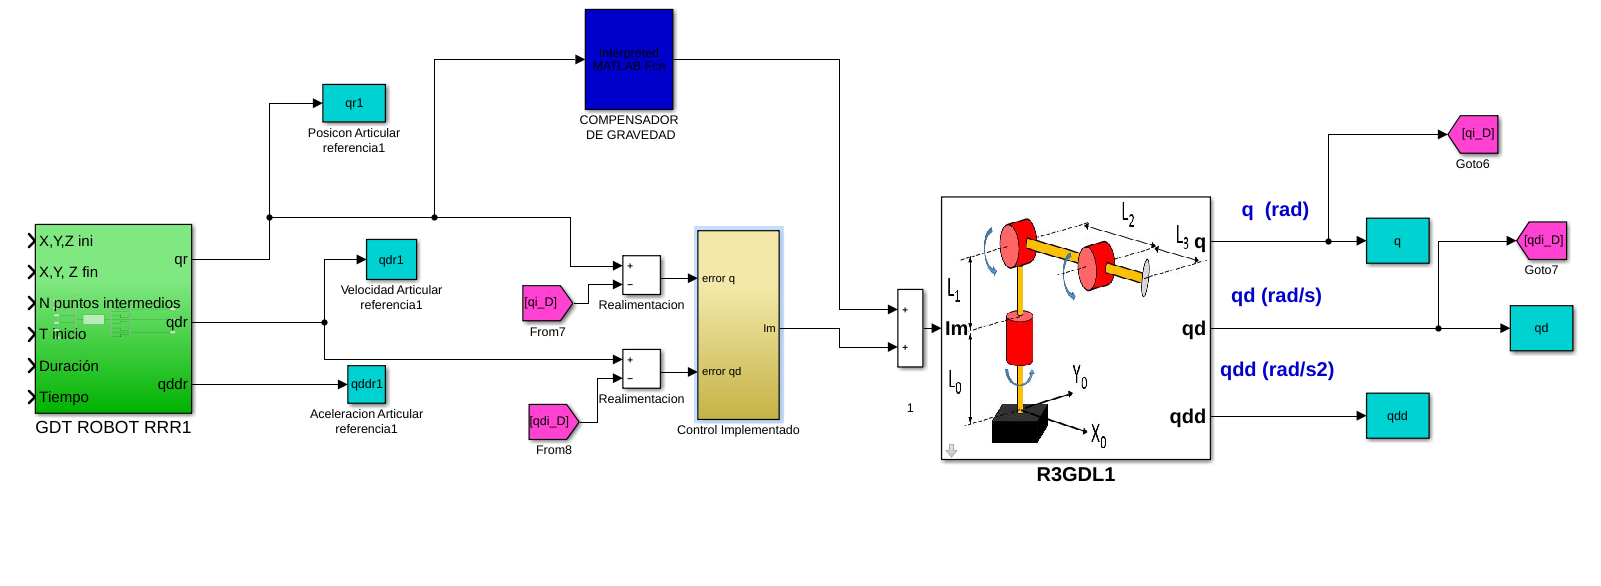
\includegraphics[width=.8\textwidth]{montaje_grav}
	\caption{Diagrama de control del compensador de gravedad}
\end{figure}

	\subsubsection{Controlador PD/PID con compensación de dinámica (Feedforward)}
	La implementación de controladores por precompensación de dinámica será la primera vez que se implementen controladores basados en modelo. La principal diferencia de éste tipo de controladores es que dependen en gran parte de la bondad del modelo obtenido, ya que se realimentará con el modelo dinámico inverso obtenido. Sin embargo, cabe destacar que en control de brazos manipuladores se emplea bastante debido a que se suele lograr obtener buenos modelos dinámicos de los robots.\\

	Para implementar éste controlador, también conocido como \textit{Feedforward}, se modificará el modelo de control de tal modo que se precompensen los efectos del modelo dinámico completo del robot, no solo la gravedad.
	\begin{equation}
		I_m= M_{A}(q)\ddot{q_{ref}} + C(q,\dot{q})\dot{q} + G_{A}(q) + u
	\end{equation}
cómo se observa, la señal de control generada estará formada por el modelo dinámico del robot más una señal adiccional,u.\\
Para conocer el valor de esa señal de control adiccional, se restará al modelo del sistema la señal de control que se desea generar de tal modo que se obtenga la expresión del bucle cerrado interno de control.
\begin{equation}
	\begin{array}{llll}
	  & Im=M_{A}(q)\ddot{q} + C_{A}(q,\dot{q})\dot{q} + G_{A}(q) \\
	- & Im=M_{A}(q)\ddot{q_{ref}} + C_{A}(q,\dot{q})\dot{q} + G_{A}(q) + u \\
	\cline{1-4}
	  & M_{A}(q)\tilde{\ddot{q}} = u & &
	\end{array}
\end{equation}
de ese modo se ha obtenido la señal de control adiccional, también conocida cómo la dinámica del error. Aunque no se lea correctamente, la ecuación obtenida es: $M_{A}(q)\tilde{\ddot{q}} = u$, dónde $\tilde{\ddot{q}}$ será el error en aceleración. \\
Habrá que diseñar controladores para la función de transferencia que se obtendrá a continuación. Para obtener dicha función de transferencia será necesario partir de condiciones iniciales nulas y transformarla al dominio de \textit{Laplace}.
\begin{equation}
	M_{A}(q)\tilde{\ddot{q}}(t) = u(t) \rightarrow M_{A}(q)\tilde{q}(s)s^{2} = u(s) \rightarrow \frac{\tilde{q}(s)}{u(s)}=\frac{K_{t}R}{M_{A}s^{2}}[\frac{ud.error}{ud.sc}]
\end{equation}

Se deberán diseñar tres funciones de transferencia, una por articulación. El esquema en diagrama de bloques de éste controlador se muestra a continuación:

\begin{figure}[h!]
	\centering
	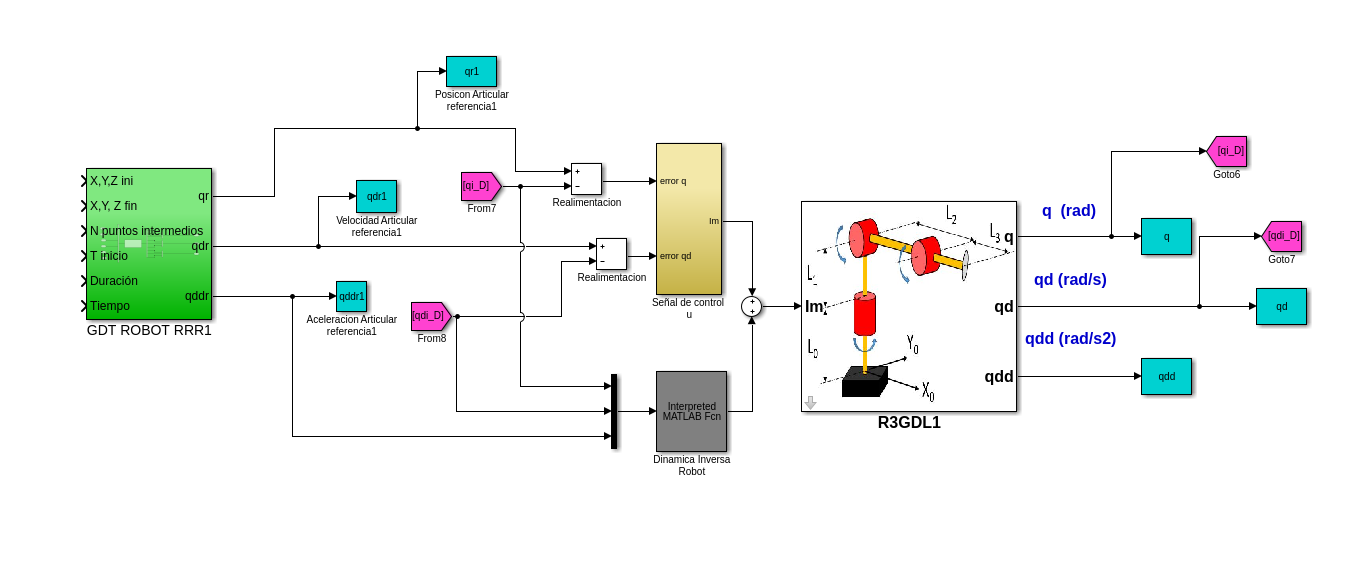
\includegraphics[width=.8\textwidth]{montaje_feedforward}
	\caption{Esquema de un controlador Feed Forward}
\end{figure}

debido a que no se puede medir la aceleración de las variables articulares, cómo se observa, el modelo dinámico inverso del robot se alimentará con los valores de las variables articulares en posición y velocidad y en el caso de la aceleración, se alimentará con la referencia obtenida del generador de trayectorias.

Por lo tanto, a modo de resumen, las funciones de transferencia de las cuales hará que obtener controladores son:
\begin{equation}
	G_{1}(s)=\frac{K_{t1}R_1}{M_{a11}s^{2}} \hspace{2cm} G_{2}(s)=\frac{K_{t2}R_2}{M_{a22}s^{2}} \hspace{2cm} G_{3}(s)=\frac{K_{t3}R_3}{M_{a33}s^{2}}
\end{equation}


	\subsubsection{Controlador PD/PID con par calculado}
	El control mediante par calculado será el último en implementar en éste proyecto. El par calculado se basa en la busqueda de desacoplar totalmente las interaciones del robot, resultando la dinámica del error cómo un doble integrador, para el cuál habrá que diseñar controladores. \\
	Que las articulaciones de un robot estén desacopladas implica que un par en un determinado actuador únicamente afectará al movimiento de dicha articulación.\\
	Por tanto, la diferencia de éste controlador frente al resto es que es un controlador dinámico. Además, es un controlador totalmente basado en el modelo, lo que conlleva que si el modelo es malo el control también lo será.
	Si, al igual que antes, se resta al sistema la señal de control que se desea implementar, se obtendrá la dinámica del error:
	\begin{equation}
		\begin{array}{llll}
		  & Im=M_{A}(q)\ddot{q} + C_{A}(q,\dot{q})\dot{q} + G_{A}(q) \\
		- & Im=M_{A}(q)(\ddot{q}_{ref}+u) + C_{A}(q,\dot{q})\dot{q} + G_{A}(q) \\
		\cline{1-4}
		\vspace{0.2cm}
		  & \tilde{\ddot{q}} = u & &
		\end{array}
	\end{equation}

	Por tanto, transformando la dinámica del error al dominio de \textit{Laplace}, las funciones de transferencia a partir de las cuales hay que diseñar los controladores serán:
	\begin{equation}
		G_{1}(s)=\frac{1}{s^{2}} \hspace{2cm} G_{2}(s)=\frac{1}{s^{2}} \hspace{2cm} G_{3}(s)=\frac{1}{s^{2}}
	\end{equation}

	Y, el esquema de control del par calculado se muestra a continuación:

		\begin{figure}[h!]
			\centering
			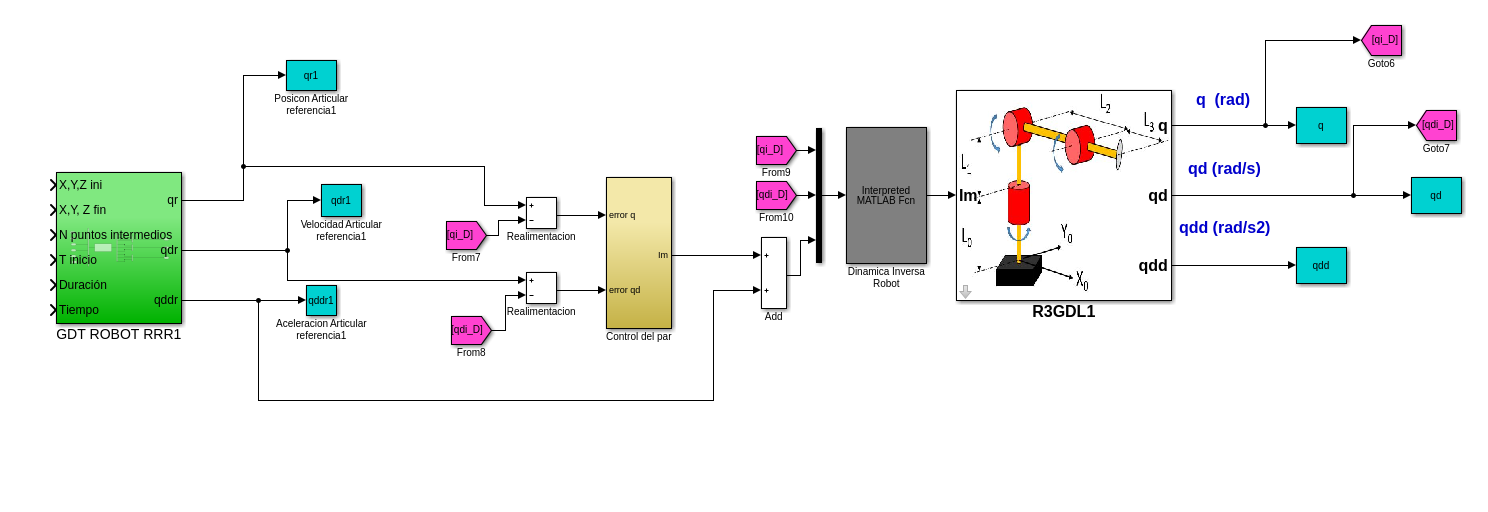
\includegraphics[width=.8\textwidth]{montaje_parcalcul}
			\caption{Esquema de un controlador Par Calculado}
		\end{figure}

\newpage
	\subsection{Analisis de experimentos para probar controladores}
En éste último apartado, se diseñarán diversos experimentos de control en los cuales se acentuen los efectos de un controlador u otro, por ejemplo, se realizarán trayectorias en las cuales se noten los efectos gravitatorios y así se observe la mejoría del controlador empleando un compensador de gravedad, etcétera.\\
Por tanto, los controladores que se van a implementar son los anteriores y los modelos a partir de los cuales se obtendrán serán el ideal y el real con y sin reductoras. También se diseñarán experimentos en el que se comparen los modelos obtenidos con medidas ideales y reales.\\

Por consiguiente, se realizarán los siguientes experimentos, en los cuales se definirá qué controladores se desea comparar y con qué fin:
\begin{itemize}
	\item En primer lugar, se realizará una comparativa entre los controladores PD y PID, de tal modo que se acentúe el efecto integral del PID y se observe la diferencia entre ambos controladores. Para ello, se generará una trayectoria relativamente lenta en la dirección negativa del eje Z, es decir, se partirá de la posición inicial del robot y se hará descender el brazo. \\

	\item Debido a que la principal perturbación que se tendrá es la gravedad, la cuál es una perturbación mantenida y conocida, la acometida del efecto integral será contrarestar ésta perturbación mantenida. Sin embargo, el principal problema del efecto integral es la agresividad del mismo. \\
	Por tanto, en éste caso, se comprobará si el error es menor al emplear un control PD con compensación de gravedad o un PID. En un ambiente real, teoricamente sería más correcto emplear el PD con la compensación para evitar los "latigazos" que podría llegar a generar en el robot el efecto integral.\\
	Seria conveniente para poder mostrar más correctamente éstos resultados buscar experimentos en los cuales se acentuen los efectos de la gravedad, para ello, lo ideal sería generar una trayectoria similar a la anterior pero en éste caso se emplearán los controladores diseñados para el robot real y se realimentarán con medidas reales. \\
	Es posible que, para mejorar el control, en lugar de realimentar el compensador de gravedad con la medida real de posición sea conveniente realimentarlo con la referencia de posición obtenida del generador de trayectorias. \\

	\item Posteriormente, se analizará el primer controlador basado en modelo, el control \textit{FeedForward}. En primer lugar sería convenientee realizar un análisis de cómo afecta la bondad del modelo a éste controlador comparando robot reales y robots ideales. \\
	Tras ello, se comprobará éste control realizando experimentos dónde se afectúen los términos de Coirolis, para ello sería conveniente realizar trayectorias ... .\\

	\item Finalmente, se analizará el controlador par calculado, el cuál se basará en desacoplar totalmente las articulaciones del robot, de tal modo que el modelo de cada articulación resulte en un doble integrador.\\
	Sería conveniente analizar trayectorias en las que se acentúen los términos inerciales del brazo robótico, ya que en éste caso se busca compensar todo el modelo.\\
	Teóricamente, si el modelo obtenido es buen modelo, debería ser el mejor controlador implementado.\\

	\item Además de todo, sería conveniente comparar el resultado del emplear una realimentación de los controladores con medidas reales o con referencia, ya que al realimentar con la referencia, se obtendrá una medida mucho más limpia y que, como es de esperar, generará un menor error. Este estudio sería conveniente en el caso de emplear los modelos con medidas reales obtenidos.\\
\end{itemize}

\newpage
\subsubsection{Comparativa controladores PD-PID ideales con reductoras}
En éste experimento, se compararán los controladores diseñados a partir del modelo ideal con reductoras. \\
La trayectoria que se empleará para éste experimentos se muestra a continuación gráficamente:
\begin{figure}[h!]
	\centering
	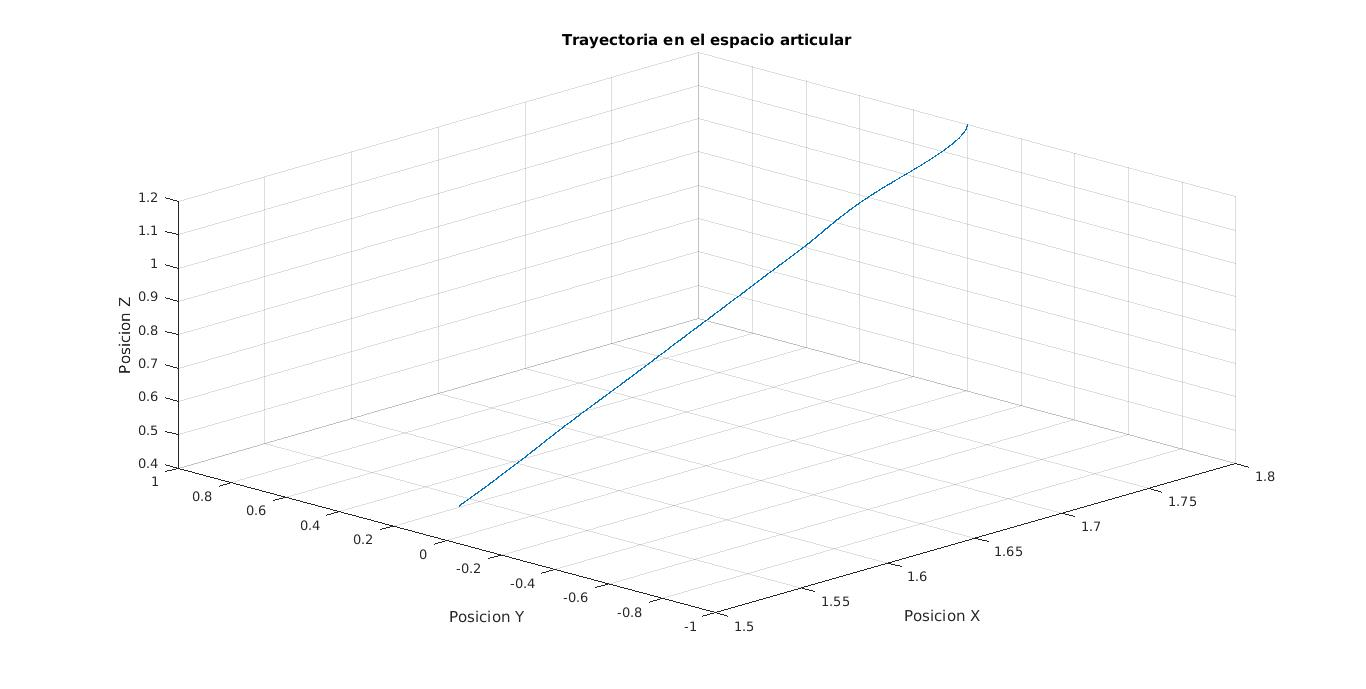
\includegraphics[width=.8\textwidth]{exp1_tray}
	\caption{Trayectoria diseñada para evaluar el efecto integral de los controladores}
\end{figure}

Cómo se ha dicho anteriormente, con éste experimento se busca evaluar el efecto integral del controlador, lo que conllevará que cuando se implemente el PID el error en regimen permamente tenderá a ser nulo, sin embargo en el caso del PD se tendrá un error mantenido.\\
Se comparará el error en posición de las tres articulaciones, ya que es dónde se observa dicho efecto:
\begin{itemize}
	\item \textbf{Controlador PD}

	\begin{figure}[h!]
		\centering
		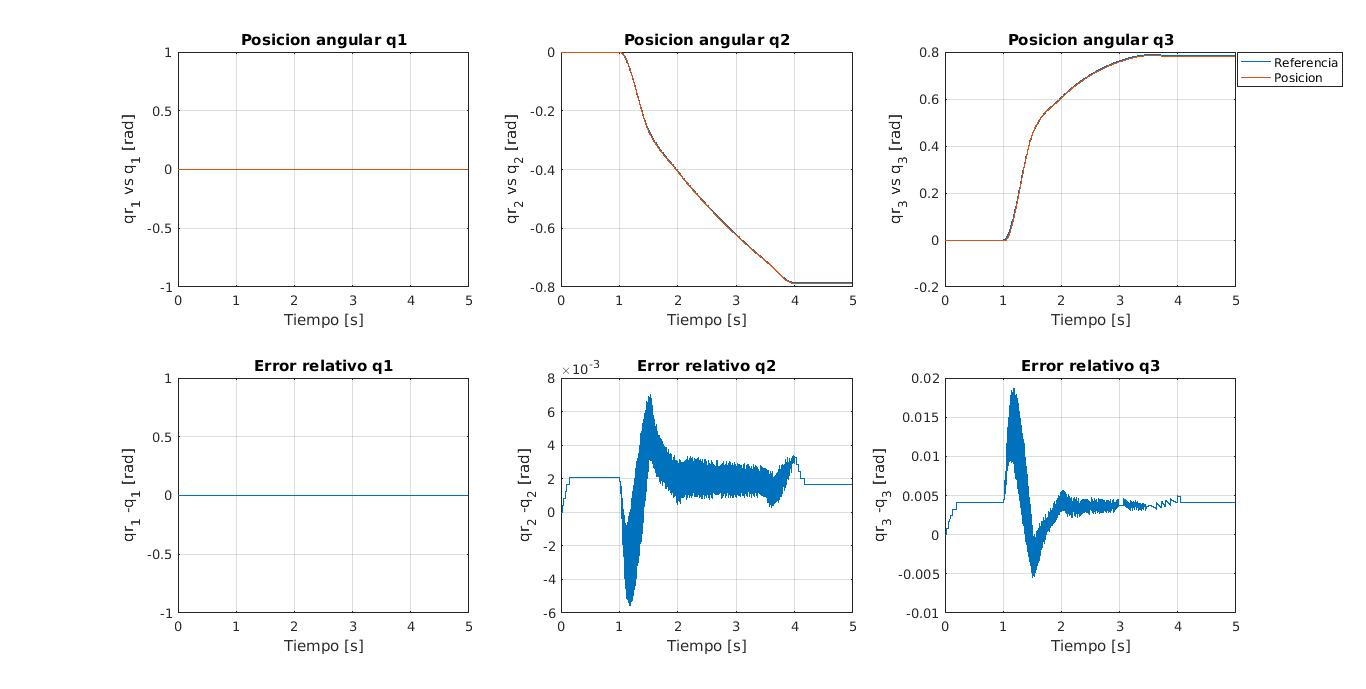
\includegraphics[width=.8\textwidth]{exp1_posPD}
		\caption{Seguimiento de referencia en posición con el controlador PD}
	\end{figure}

\newpage
	\item \textbf{Controlador PID}
	\begin{figure}[h!]
		\centering
		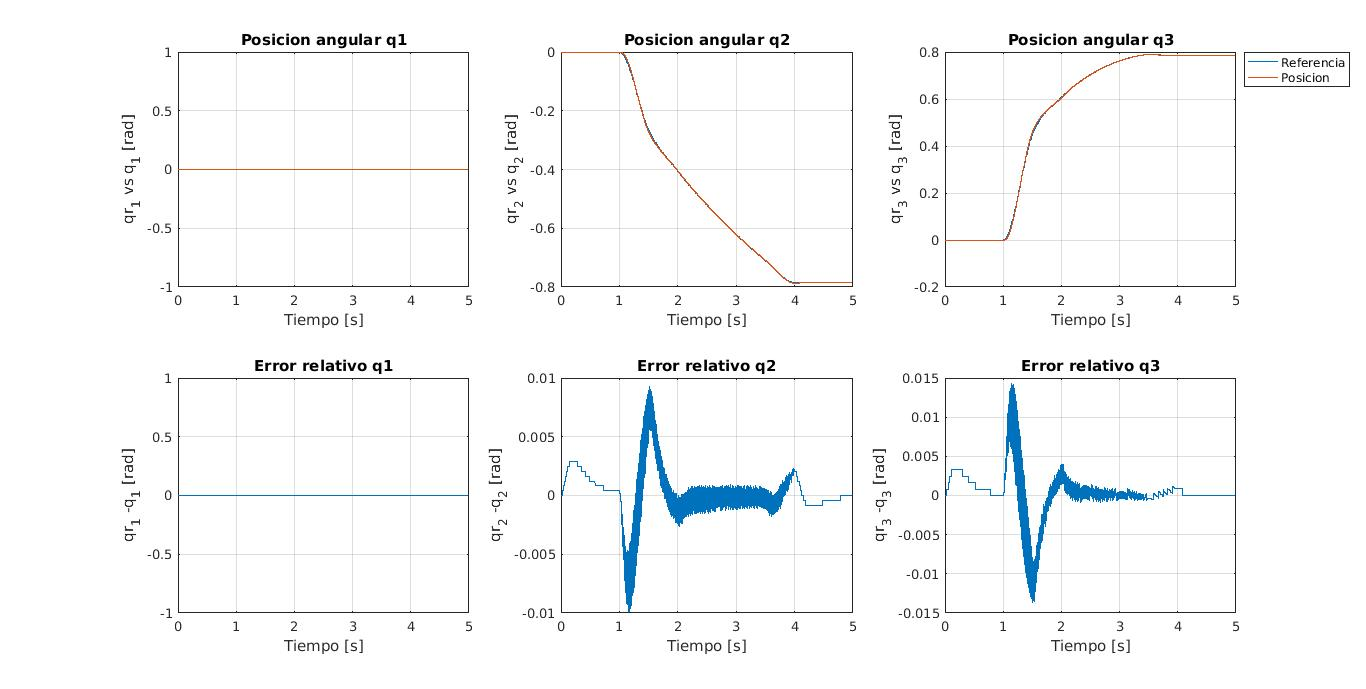
\includegraphics[width=.8\textwidth]{exp1_posPID}
		\caption{Seguimiento de referencia en posición con el controlador PID}
	\end{figure}

\end{itemize}

Se observa claramente cómo el efecto integral compensa la perturbación mantenida que es la gravedad, por tanto, el controlador PID mejora la respuesta del PD asumiento la agresividad del efecto integral.

\newpage
\subsubsection{Comparativa controlador PID y PD con compensacion gravedad}
En éste caso, se implementarán los controladores diseñados en base al modelo del robot real con reductoras. Debido a que se han empleado medidas reales, se realimentarán con las medidas reales del robot. Si la respuesta no fuese lo suficientemente aceptable, se alimentaría el compensador de gravedad con la referencia obtenida del generador de trayectorias. \\
Se ha optado por emplear la misma trayectoria que anteriormente debido a que se busca que se acentuen los efectos asociados a los terminos gravitatorios, al igual que antes.\\
\begin{itemize}
	\item \textbf{Mejora del resultado obtenido con el controlador anterior} \\
Si se compara el resultado obtenido anteriormente con el PID a partir del modelo ideal con el resultado obtenido al implementar un controlador PD con compensador de gravedad, se observa que éste segundo nos dará unos mejores resultados en el seguimiento de la trayectoria y una menor magnitud del error. La grafica de seguimiento se muestra a continuación:

\begin{figure}[h!]
	\centering
	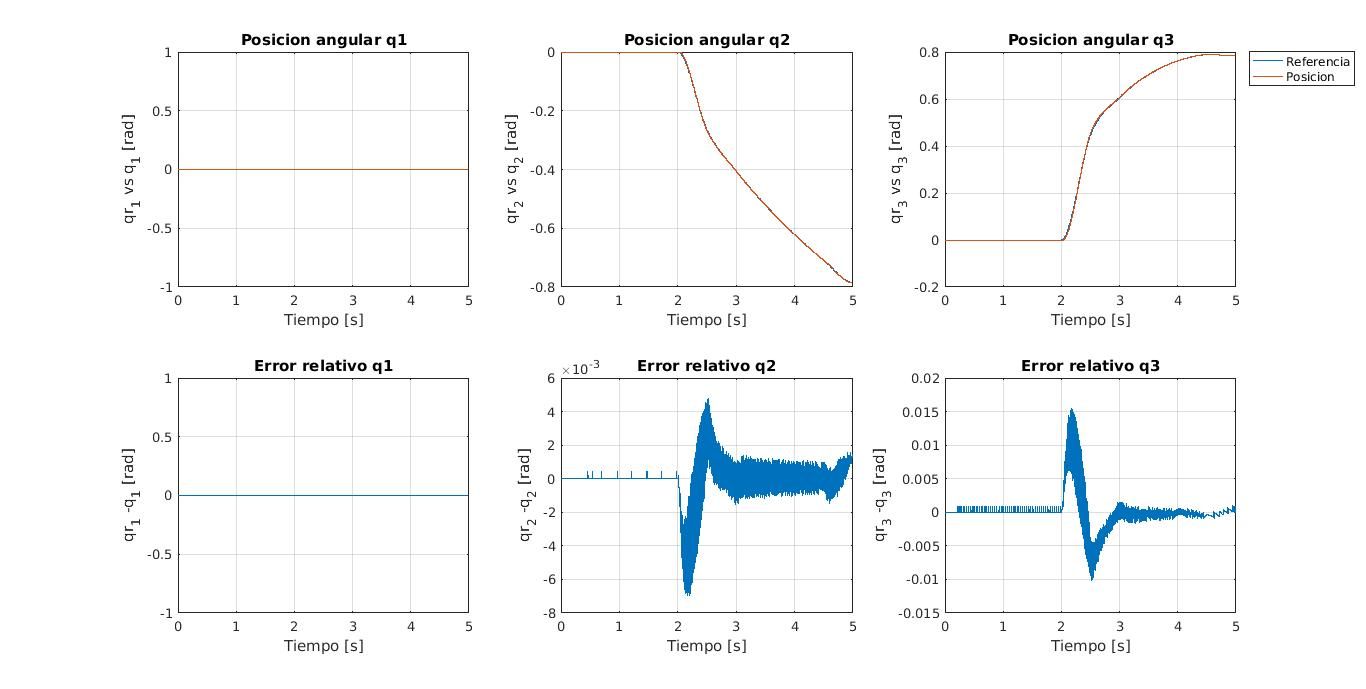
\includegraphics[width=.8\textwidth]{exp2_posPDcomp}
	\caption{Seguimiento de referencia en posición con el controlador PD con compensación de gravedad}
\end{figure}

%Si en lugar de realimentar el compensador con la medida real de posición, es decir, la que se obtiene de los encoders, se realimenta con %la referencia que dá el generador de trayectorias el resultado es notablemente mejor, ésto es debido a que se está realimentando con una %señal límpia.
\end{itemize}

\newpage
\subsubsection{Comparativa del control con compensación de dinámica o \textit{FeedForward}}
En éste apartado, se comprobará la bondad de los modelos obtenidos. Para ello, implementará la primera técnica de control avanzado que se dispone, la cuál es el control con compensación de dinámica.\\
Por tanto, para éste controlador se diseñará un controlador PD o PID que compense la dinámica del error y se compensará la dinámica del robot, en concreto los términos de Coirolis.\\

Se deberá buscar un experimento en el cuál se acentúen los terminos de Coirolis, por ello se ha optado por emplear el que se muestra a continuación, el cuál es un movimientos que contiene giro sobre la base en un tiempo medio, es decir, ni excesivamente rápido ni lento. \\
La trayectoria que se empleará para éste experimento partirá de las variables articulares nulas y girará sobre sí mismo bajando el brazo, intentando acentuar los términos de Coirolis.\\

Inicialmente, se comparará la bondad de los modelos obtenidos con reductoras. Por tanto, a continuación se mostrará el seguimiento de la trayectoria en el plano XYZ y el seguimiento de la referencia en posición de las variables articulares, tras ello, se sacarán una serie de conclusiones:
\begin{itemize}
	\item \textbf{Robot ideal con reductoras} \\
	El seguimiento de la trayectoria en el plano XYZ será:
	\begin{figure}[h!]
		\centering
		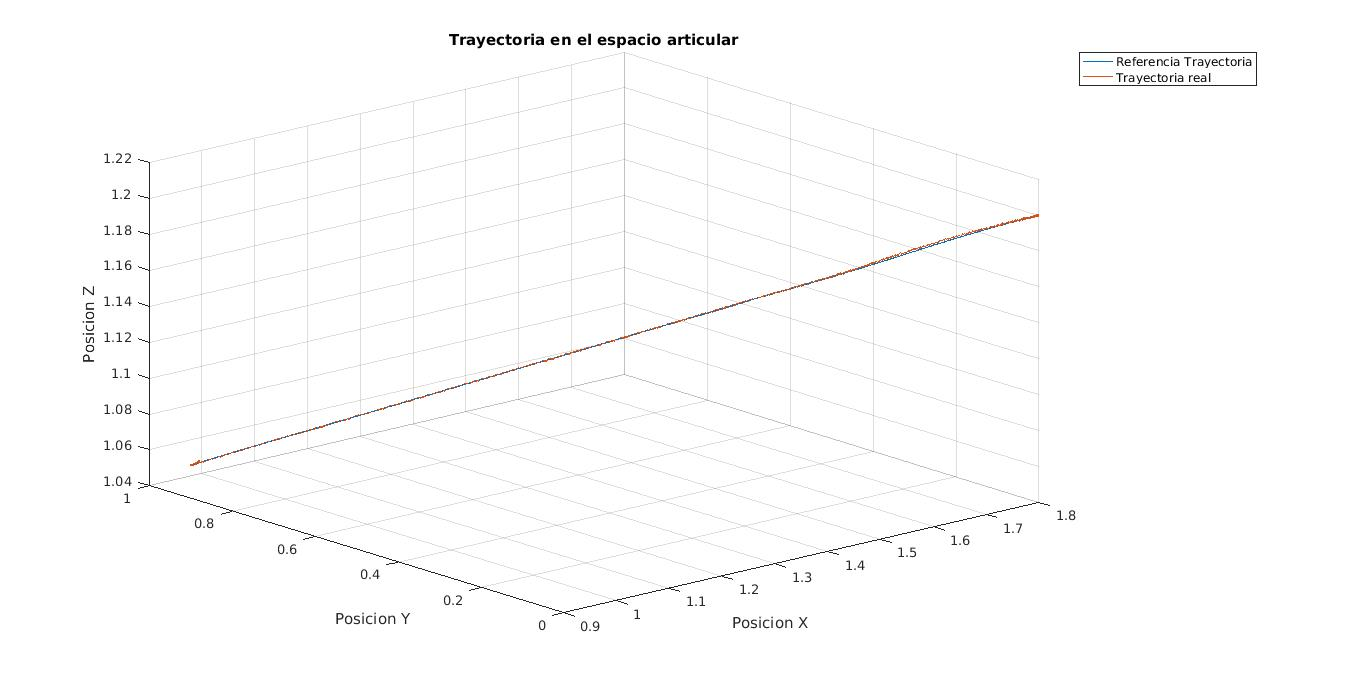
\includegraphics[width=.7\textwidth]{exp3_trayPDideal}
		\caption{Seguimiento de la trayectoria en el plano XYZ}
	\end{figure}

	Se observa cómo, a primera vista, se ha obtenido un buen modelo, ya que el seguimiento será bastante bueno. A continuación se verá cómo siguen la referencia de posición las variables articulares del robot:

	\begin{figure}[h!]
		\centering
		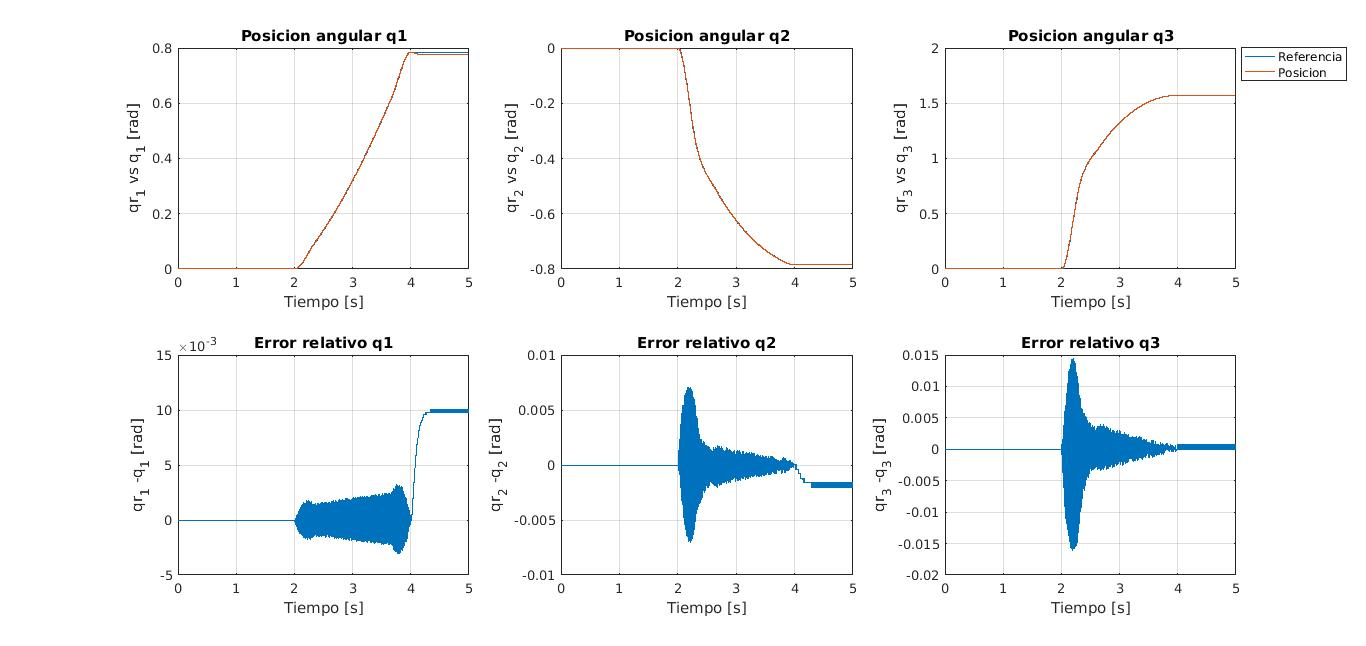
\includegraphics[width=.8\textwidth]{exp3_posPDidealCR}
		\caption{Seguimiento de referencia en posición de las variables articulares}
	\end{figure}


	Aunque se aprecia un cierto error, la magnitud de éste es pequeña y, por tanto, fácilmente asumible. También cabe destacar que, la segunda articulación quizá se haya estimado algo peor, ya que es la que presenta error en regimen permanente tras la trayectoria. \\

	\item \textbf{Robot real con reductoras} \\
	El seguimiento de la trayectoria en el plano XYZ será:

	\begin{figure}[h!]
		\centering
		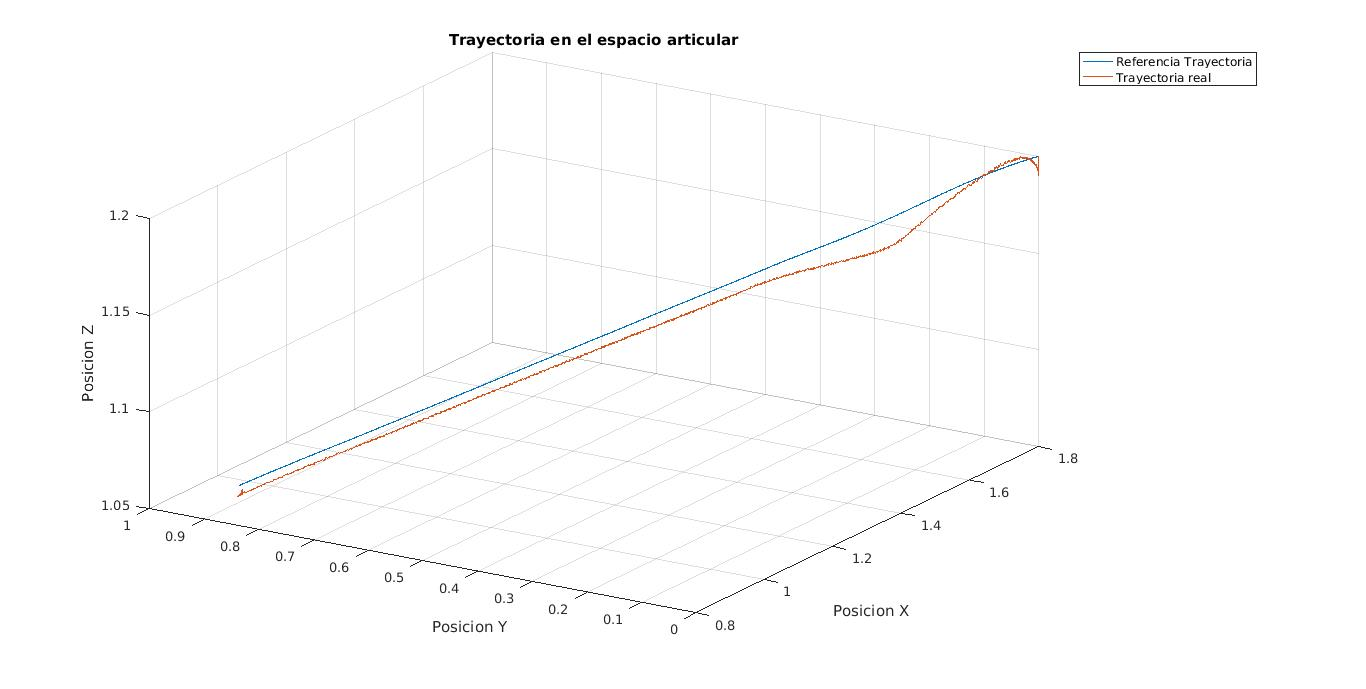
\includegraphics[width=.8\textwidth]{exp3_trayPDreal}
		\caption{Seguimiento de la trayectoria en el plano XYZ}
	\end{figure}

	En éste caso, debido a que se han tomado medidas reales para obtener el modelo del robot, se observa que se tendrá un error mantenido en el seguimiento de la trayectoria en el plano XYZ. Para analizar con mayor exactitud dicho error, es conveniente observar el seguimiento a referencia en posición realizado por las variables articuales del robot:

	\begin{figure}[h!]
		\centering
		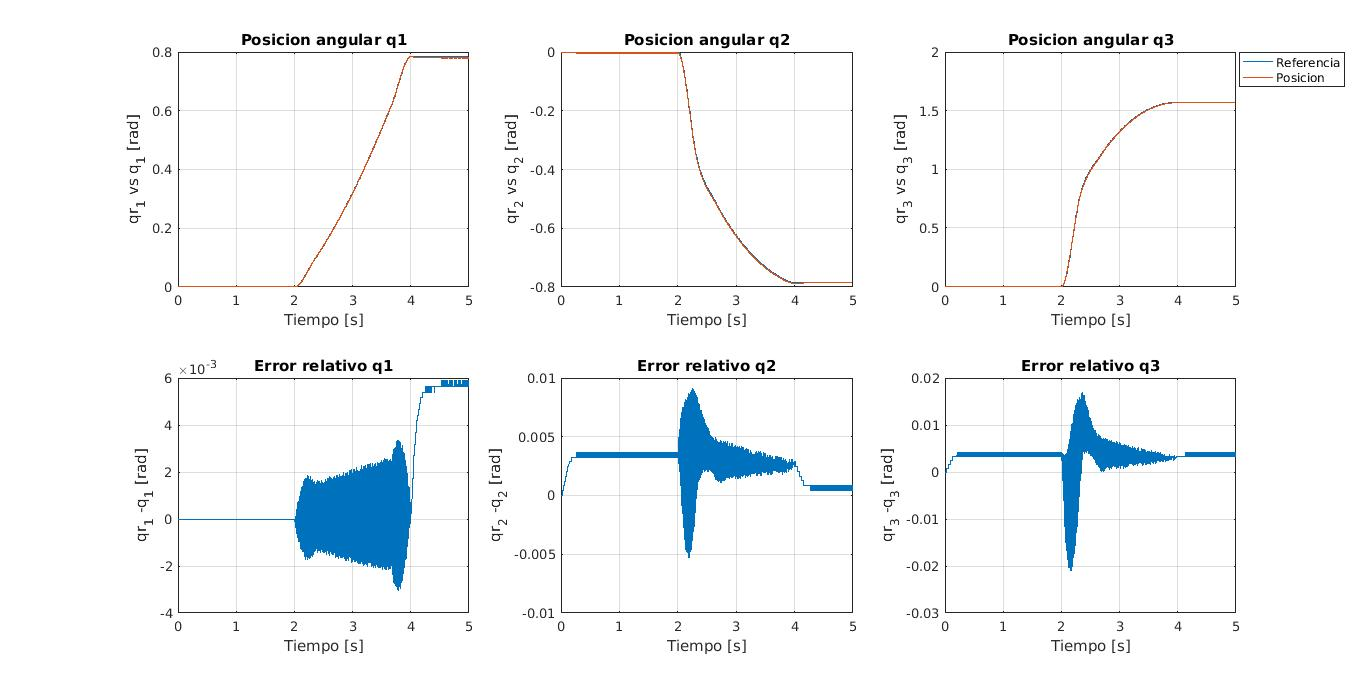
\includegraphics[width=.8\textwidth]{exp3_posPDrealCR}
		\caption{Seguimiento de referencia de las variables articulares}
	\end{figure}

Se puede observar que todas las variables articulares tras la trayectoría presentarán un error mantenido, sin embargo, la magnitud del mismo será pequeña.\\
Por tanto, se puede estimar que no se ha obtenido un mal modelo real del robot con reductoras, aunque no es perfecto, ni tan bueno cómo el ideal, será un modelo válido para trabajar con el mismo.

\end{itemize}

Otro buen experimento para probar éste controlador será la generación de trayectorias curvas, ya que se podrá llegar a acenturar los términos de Coirolis. Se ha optado por una trayectoria no muy rápida pero que sí recorra algo mas que media circunferencia, de tal modo que puedan llegar a obtenerse resultados concluyentes. Al igual que antes, se comparará la respuesta del robot a partir del controlador diseñado en base al modelo real con el diseñado en base al modelo ideal. \\
\begin{itemize}
	\item \textbf{Robot Real con reductoras} \\
La trayectoria a seguir por el robot en el plano XYZ se muestra a continuación:

\begin{figure}[h!]
	\centering
	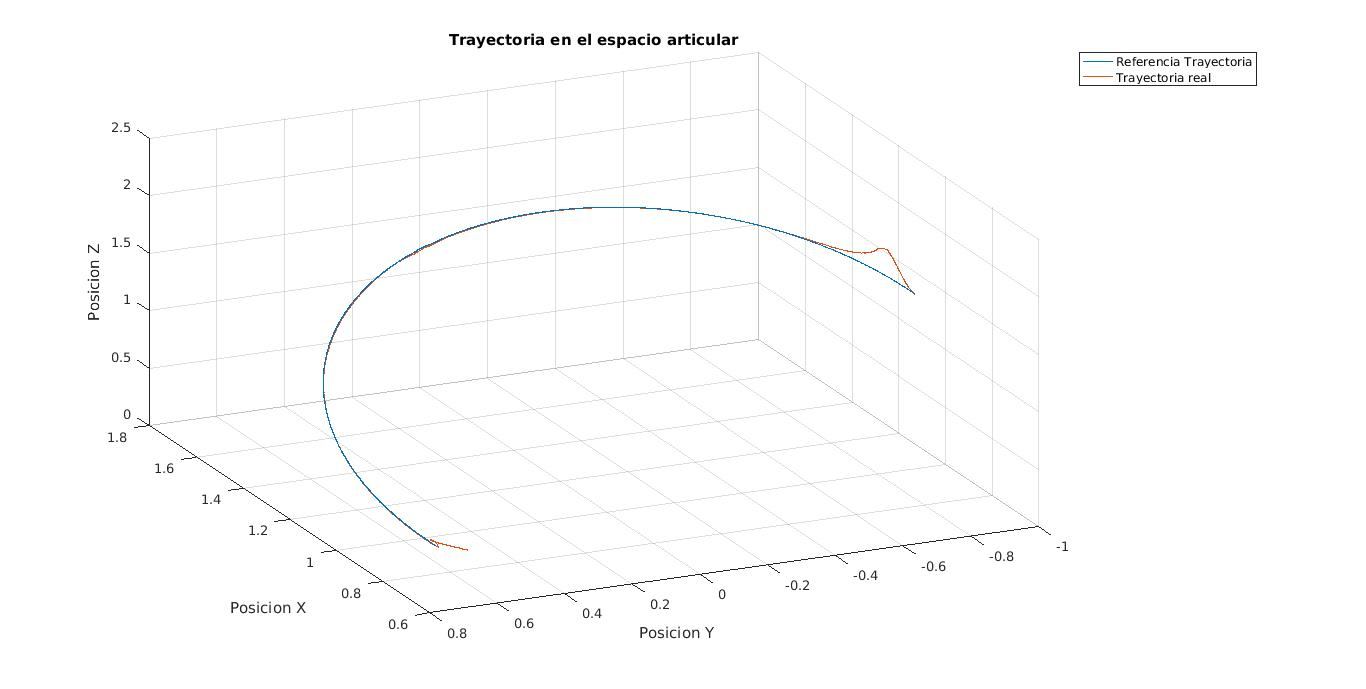
\includegraphics[width=.8\textwidth]{exp3_trayPDreal_circular}
	\caption{Referencia y seguimiento de trayectoria en el plano XYZ}
\end{figure}

Se obseva que va a aparecer un error en la trayectoria, además será un error mantenido. En el caso del seguimiento de referencia en las variables articulares, el resultado obtenido es:

\begin{figure}[h!]
	\centering
	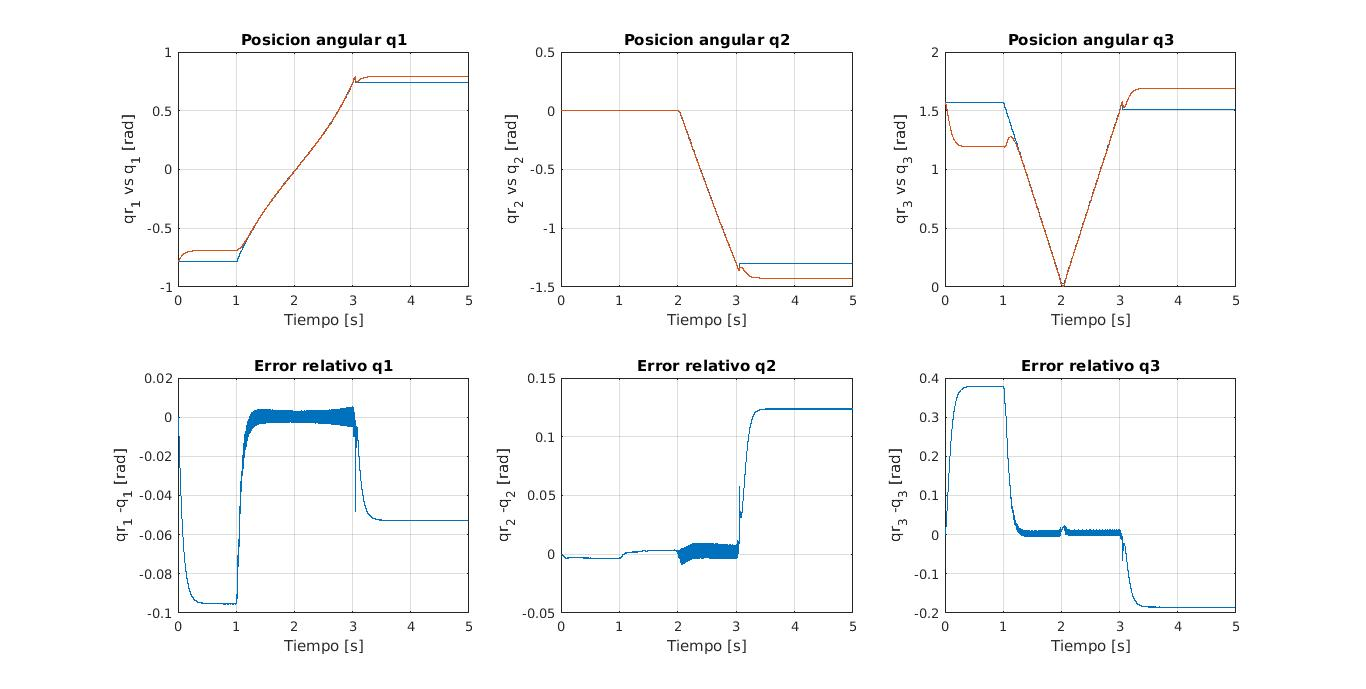
\includegraphics[width=.8\textwidth]{exp3_posPDrealCR_circular}
	\caption{Seguimiento de referencia de las variables articulares}
\end{figure}

Se observa que hay un error mantenido, el cual podría llegar a no ser asumible. Por tanto, se optará por emplear el modelo ideal obtenido del robot y en aumentarle el tiempo en el que tiene que hacer la trayectoria, en post de minimizar el error del robot.


	\item \textbf{Robot Ideal con reductoras} \\
En éste caso, al haber empleado más tiempo para seguir la trayectoria y el modelo ideal del robot, los errores cometidos por el robot, aunque siguen existiendo, han decrementado su magnitud cómo puede verse a continuación:

\begin{figure}[h!]
	\centering
	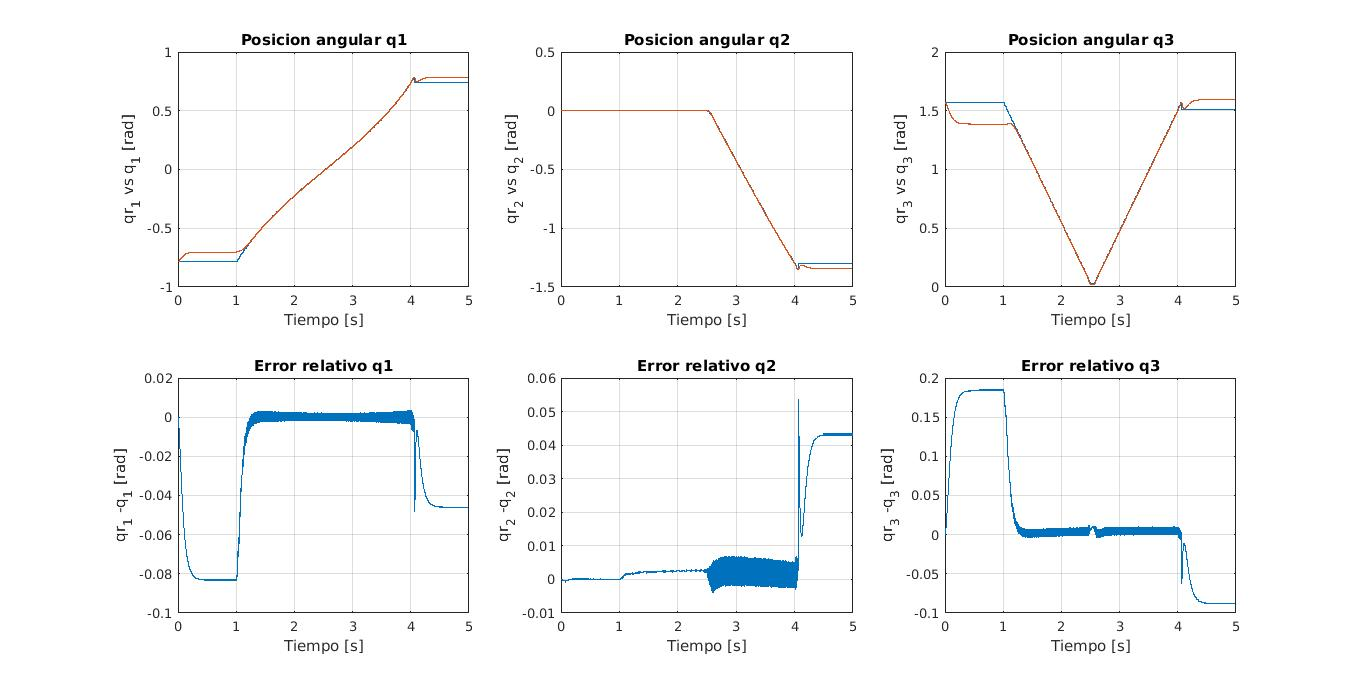
\includegraphics[width=.8\textwidth]{exp3_posPDidealCR_circular_lento}
	\caption{Seguimiento de referencia de las variables articulares}
\end{figure}

\end{itemize}

\newpage
\subsubsection{Comparativa del control par calculado}
En el controlador mediante par calculado se ha desacoplado totalmente las articulaciones del robot, de tal modo que la dinámica del error resultante es un doble integrador. \\
Además de ello, se notará más éste controlador cuando se trabaje sin reductoras, ya que las reductoras son las encargadas de desacoplar las articulaciones del robot, por tanto, si no se emplean reductoras, el encargado de desacoplar las articulaciones será el propio control implementado. \\
Además de ello, también se buscará mostrar que, cuán más rápido se busque que sea el control, mayores serán los errores que se tendrán.\\

Por tanto, en primer lugar se empleará el robot ideal sin reductoras para mostrar el efecto de pedir mayor velocidad en el movimiento del robot y, posteriormente, se comparará el modelo ideal sin reductoras y el modelo real sin reductoras.\\
La trayectoria elegida será una trayectoria ascendente y de rotación que partirá de la posición inicial del robot.

\begin{itemize}
	\item \textbf{Comprobación del efecto del aumento de la velocidad en la trayectoria} \\
	A continuación, en primer lugar se mostrará la comparativa del seguimiento de la trayectoria en el espacio articular XYZ en función del la velocidad pedida para que siga la misma. Además, cabe destacar que se ha implementado un control PD para la dinámica del error.\\
	En primer lugar se mostrará la gráfica en la que se pedía que recorriese la trayectoria en 2 segundos, es decir, la que sería la trayectoria lenta:

	\begin{figure}[h!]
		\centering
		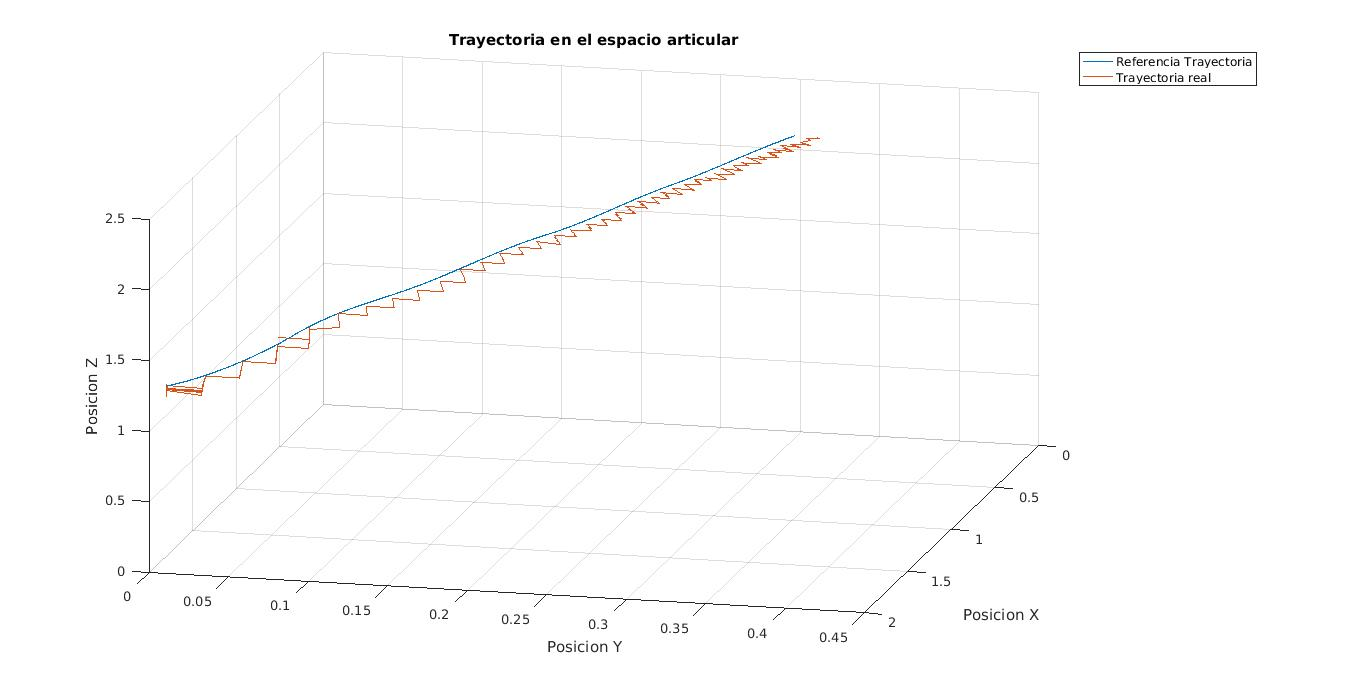
\includegraphics[width=.8\textwidth]{exp4_trayPDidealSR_lento}
		\caption{Seguimiento de la trayectoria lenta en el plano XYZ}
	\end{figure}

	Ahora, se mostrará el seguimiento en posiciones articulares cuando se pide que se siga la trayectoria algo más lenta:

	\begin{figure}[h!]
		\centering
		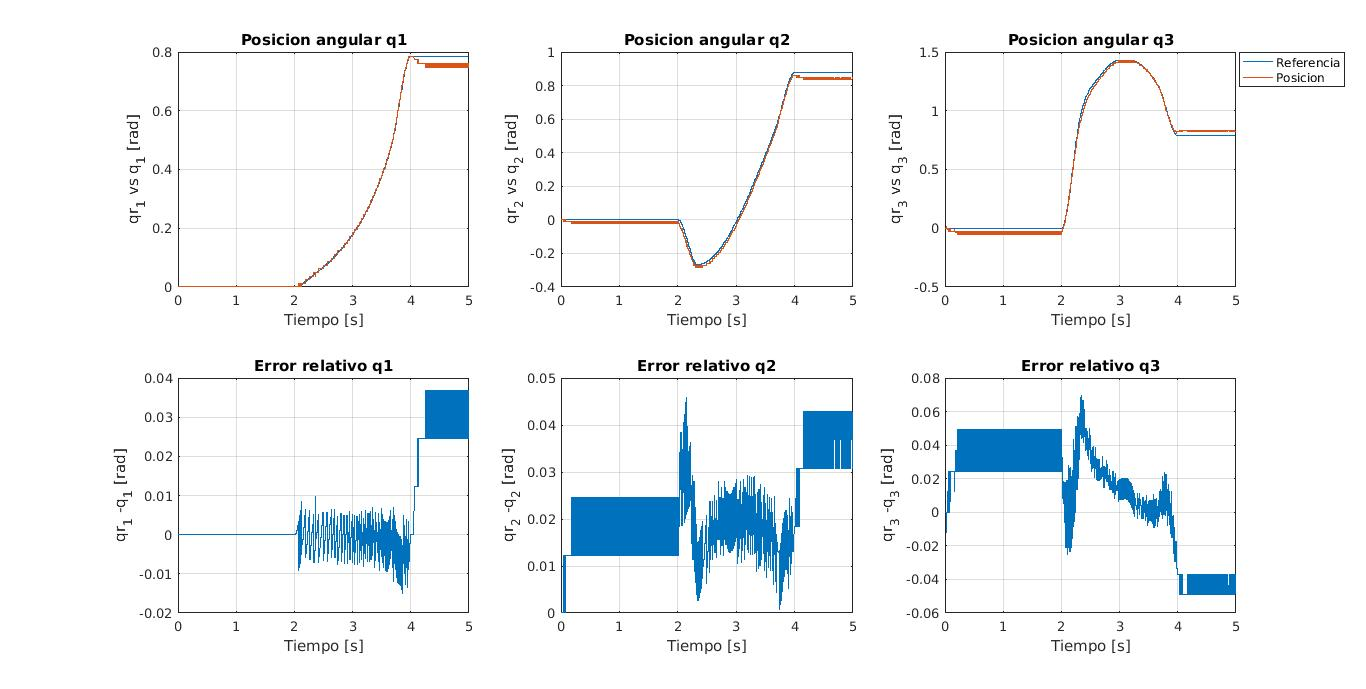
\includegraphics[width=.8\textwidth]{exp4_posPDidealSR_lento}
		\caption{Seguimiento de las variables articulares}
	\end{figure}

\newpage
Se observa que, aunque existe un error en las tres variables, éste error es significativamente pequeño y asumible en el control del robot.\\
Sin embargo, en el caso de que se pida que realice la trayectoria en la mitad de tiempo, el error se incrementará significativamente cómo se muestra a continuación:

\begin{figure}[h!]
	\centering
	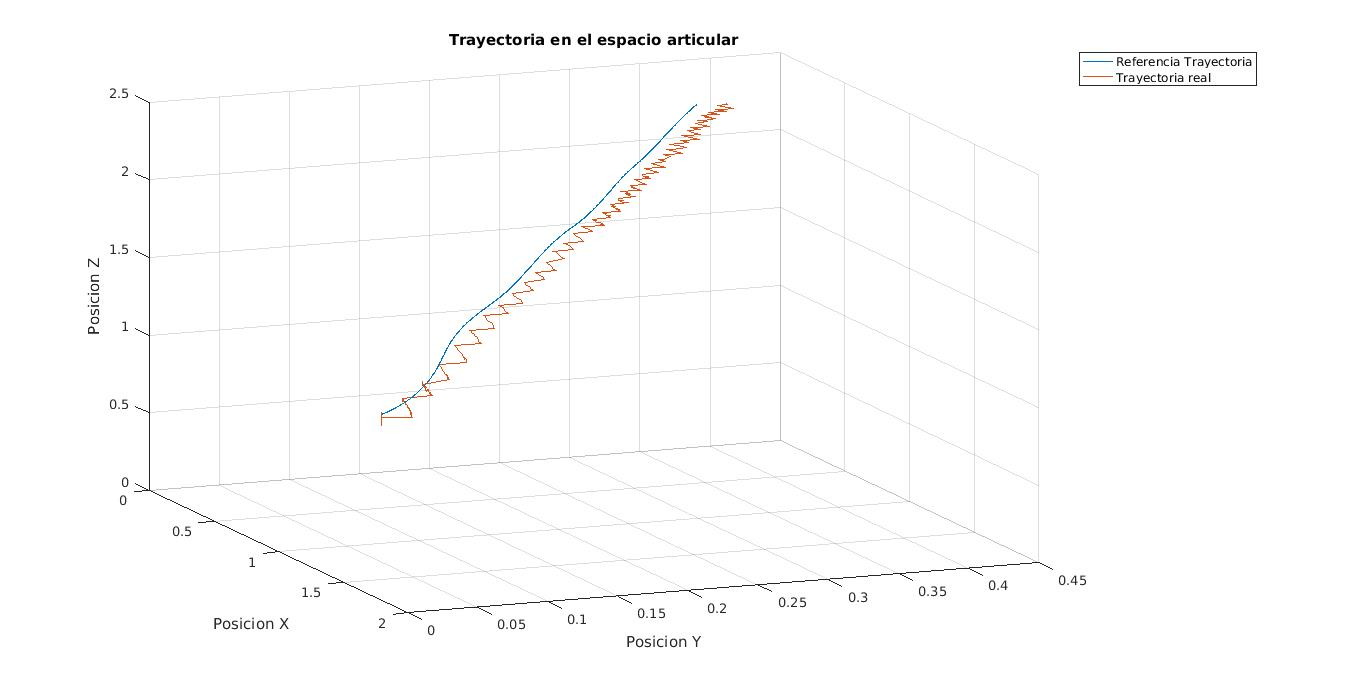
\includegraphics[width=.8\textwidth]{exp4_trayPDidealSR_rapido}
	\caption{Seguimiento de la trayectoria rapida en el plano XYZ}
\end{figure}

\newpage
Ahora, se mostrará el seguimiento en posiciones articulares cuando se pide que se siga la trayectoria en el doble de tiempo:

\begin{figure}[h!]
	\centering
	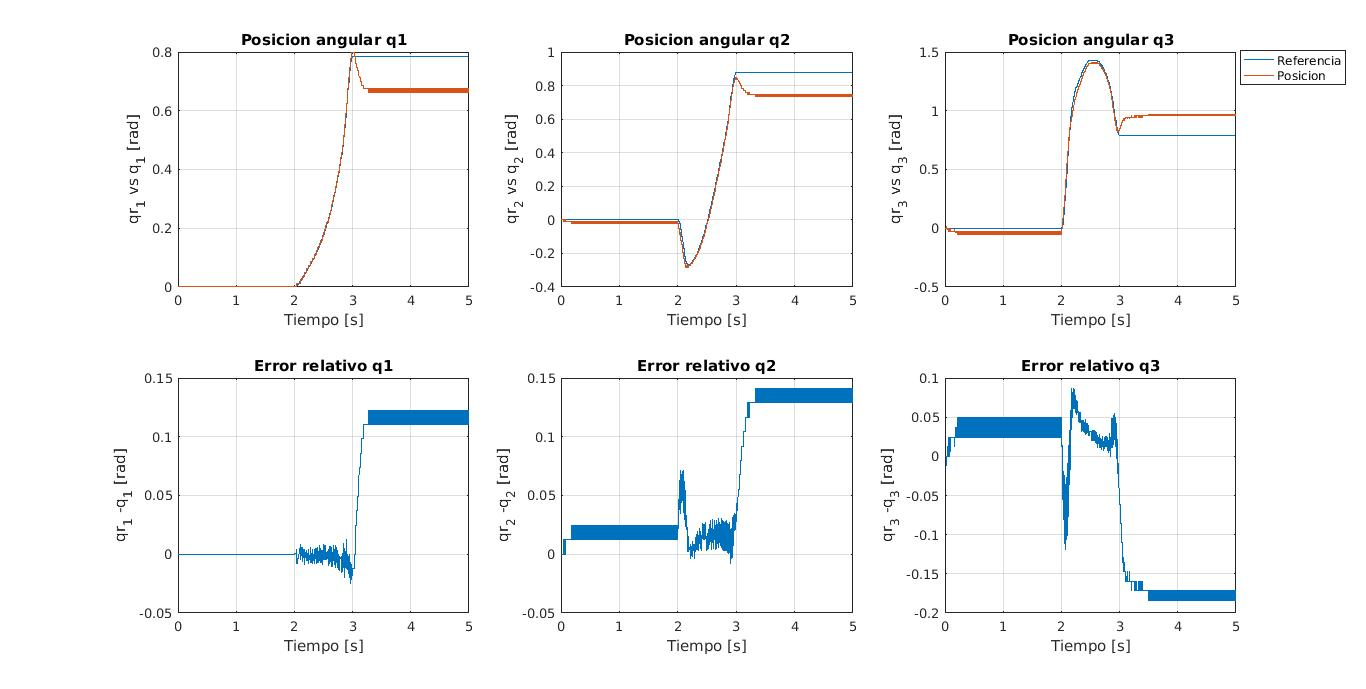
\includegraphics[width=.8\textwidth]{exp4_posPDidealSR_rapido}
	\caption{Seguimiento de las variables articulares}
\end{figure}

Por tanto, a modo de conclusión cabe destacar que, en el momento de pedirle al robot que siga una trayectoría será necesario hayar un compromiso entre la velocidad de la trayectoria y el error que se esté dispuesto a asumir en la misma.\\

	\item \textbf{Comparativa del modelo ideal sin reductoras obtenido y el real} \\
Para comprobar la bondad del modelo real sin reductoras obtenido, se trazará con éste la primera trayectoria descrita en éste apartado, es decir, la que va mas despacio y de ese modo, se podrá ver de manera significativa la comparativa entre el modelo ideal sin reductorias y el modelo real sin reductoras obtenido. \\
Por tanto, en el espacio la trayectoria seguida empleando el control par calculado con el modelo real sin reductoras se muestra a continuación. Cabe destacar que éstas gráficas han sido obtenidas realimentando el control con la referencia de posición y de velocidad, no con las medidas tomadas del robot, ya que de ese modo se evita tener medidas tan ruidos y se puedes estimar mejor los resultados.\\
Posteriormente se observará cómo sería el resultado si se hubiese realimentado con las medidas tomadas del robot.\\

Debido a que el modelo obtenido se degrada con el tiempo, es decir, cuanto mas tiempo de simulación pasa mayores serán los errores, hay un punto en el cuál el sistema se hará inestable, ya que en éste tipo de control se depende totalmente del modelo obtenido, cómo se muestra a continuación:

\begin{figure}[h!]
	\centering
	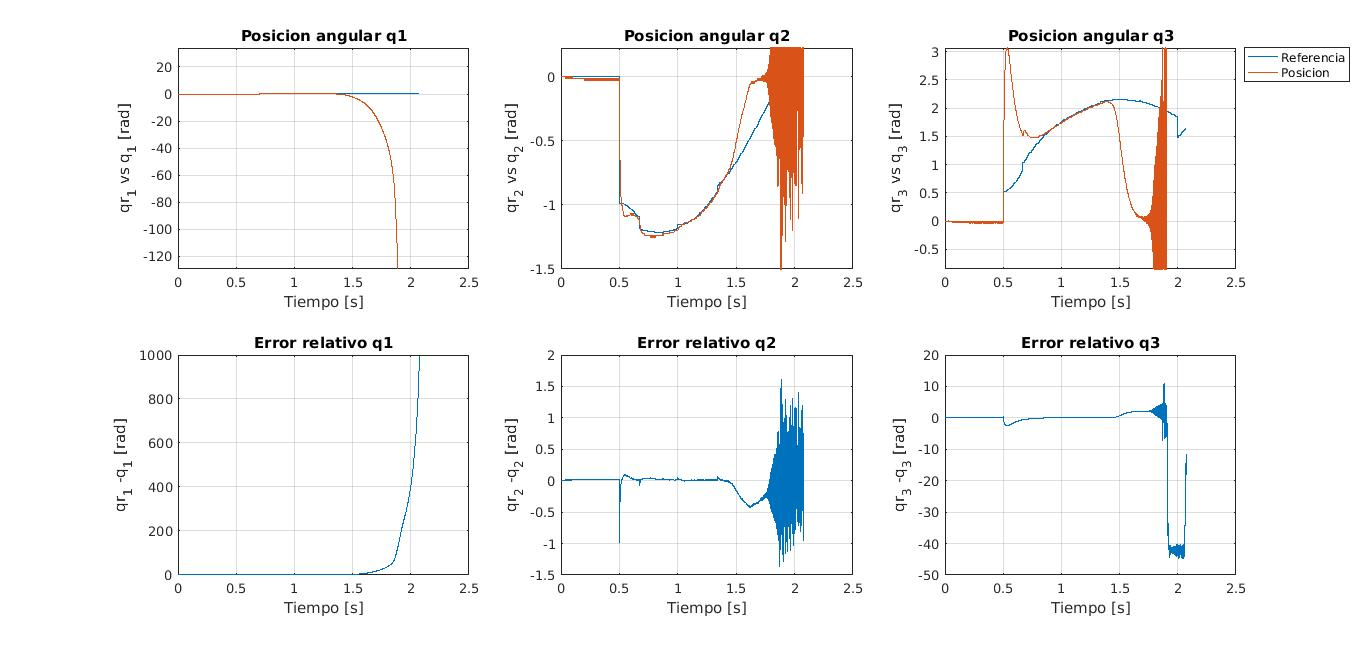
\includegraphics[width=.8\textwidth]{exp4_posPDrealSR}
	\caption{Seguimiento de las variables articulares}
\end{figure}

\end{itemize}
